\begin{figure}[h!]
    \centering
    \caption{Desempenho dos modelos de regressão aplicados para inferir as leituras de concentração de \acrshort{mp10} medidas pela estação de referência}
    \begin{subfigure}{0.9\textwidth}
        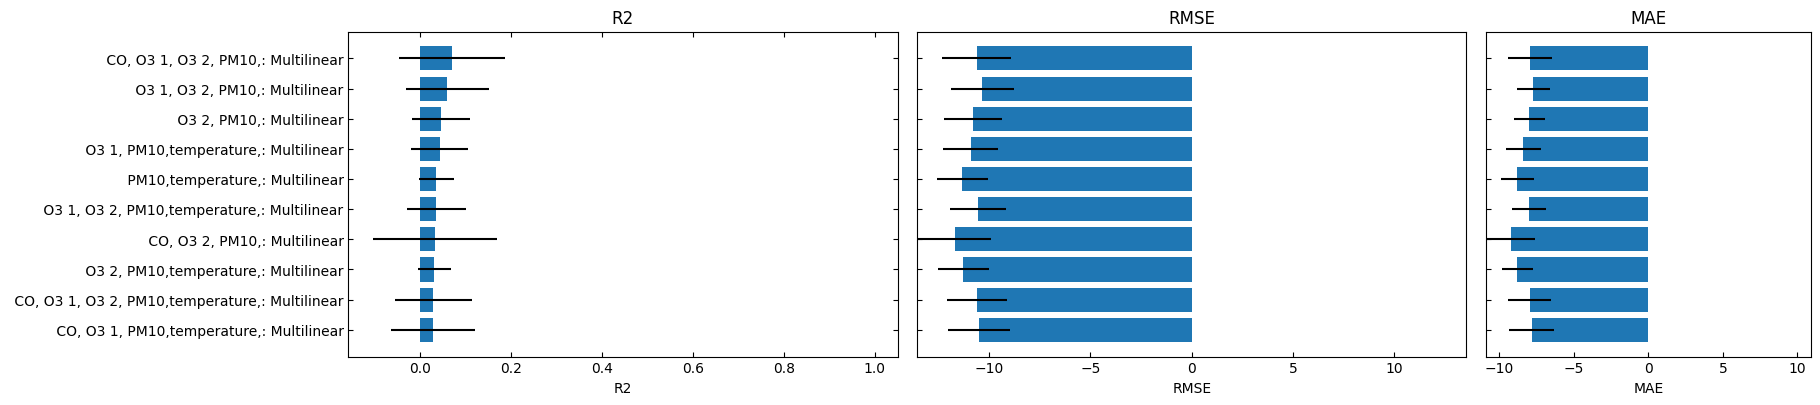
\includegraphics[width=\textwidth]{chapters/4-CALIBRAÇÃO MÚLTIPLOS SENSORES/Figuras/pm10-all-models-performance.png}
        \caption{Valores de R2, RMSE e MAE obtidos pelos 10 modelos com maiores valores de R2}
        \label{fig:data-pm10-all-models-performance}
    \end{subfigure}
    \begin{subfigure}{0.9\textwidth}
        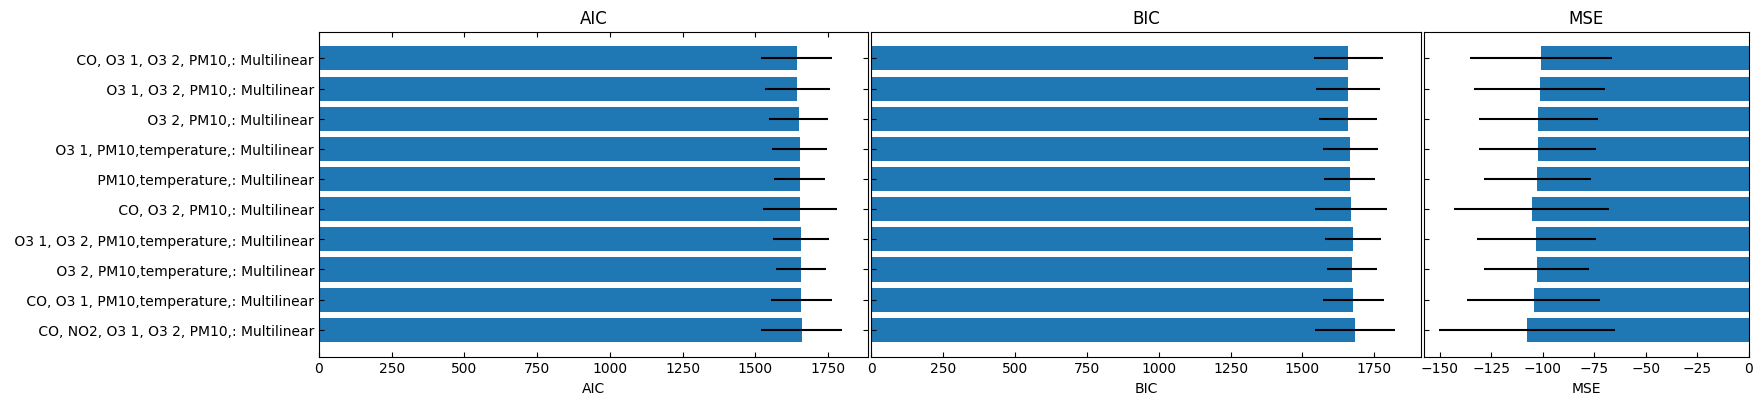
\includegraphics[width=\textwidth]{chapters/4-CALIBRAÇÃO MÚLTIPLOS SENSORES/Figuras/pm10-all-models-complexity.png}
        \caption{Modelos com menores valores de \acrshort{aic} e \acrshort{bic}}
        \label{fig:data-pm10-all-models-comlexity}
    \end{subfigure}
    \label{fig:data-pm10-all-models-performance-comlexity}
\end{figure}

% ----------------------------------------------------------
\section{Calibração das leituras de Material Particulado }
% ----------------------------------------------------------

A Figura \ref{fig:data-pm10-all-models-performance} apresenta os valores de R2 dos 10 melhores modelos de calibração calculados para as leituras de \acrshort{mp10}. Observa-se que os valores de R2 desses 10 modelos apresentaram valores de R2 em média positivos, com valores mínimos e máximos oscilando entre -0.1 e 0.2, todos obtidos a partir de regressões lineares. Com relação as variáveis de entrada observa-se maior variabilidade do que nos casos analisados anteriormente, mas em geral destaca-se a presença de sensores de \acrshort{o3} em 9 dos modelos e em segundo lugar da temperatura, presente em 6. Nenhum dos modelos incluiu leituras do sensor NO2-B43F. Com relação à complexidade dos modelos (Figura \ref{fig:data-pm10-all-models-performance-comlexity}) observa-se bastante coincidência com ranqueamento de R2. As Figuras \ref{fig:data-co-o31-o31-pm10-reference-PM10-corr-MLR} e \ref{fig:data-o31-o32-pm10-reference-PM10-corr-RF} mostram os resultados obtidos com os dois modelos com maior R2 médio, i.e.: regressões lineares com variáveis de entrada leituras de sensores CO-B4, OX-B431 (1 e 2) e sensor de \acrshort{mp10} OPC-N3, e leituras de sensores OX-B431 (1 e 2) e sensor de \acrshort{mp10} OPC-N3, respectivamente. As figuras mostram gráficos de dispersão entre os dados calibrados por esses modelos e as leituras de referência.

\begin{figure}[h]
    \centering
    \caption{Gráfico de dispersão das leituras do múltiplos sensores e a estação de referência para medição de \acrshort{mp10}}
    \begin{subfigure}{0.49\textwidth}
        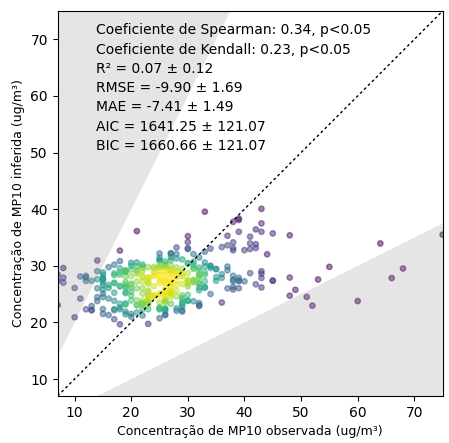
\includegraphics[width=\textwidth]{chapters/4-CALIBRAÇÃO MÚLTIPLOS SENSORES/Figuras/MP10-co-o31-o32-pm10-Multilinear-Regression.png}
        \caption{Utilizando modelo de regressão linear multivariado com variáveis independentes: leituras de sensores CO-B4, OX-B431 (1 e 2) e sensor de \acrshort{mp10} OPC-N3}
        \label{fig:data-co-o31-o31-pm10-reference-PM10-corr-MLR}
    \end{subfigure}
    \hfill
    \begin{subfigure}{0.49\textwidth}
        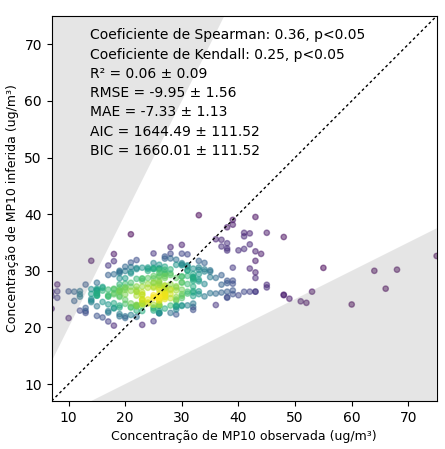
\includegraphics[width=\textwidth]{chapters/4-CALIBRAÇÃO MÚLTIPLOS SENSORES/Figuras/MP10-o31-o32-pm10-Multilinear-Regression.png}
        \caption{Utilizando modelo de regressão linear multivariado com variáveis independentes: leituras de sensores OX-B431 (1 e 2) e sensor de \acrshort{mp10} OPC-N3}
        \label{fig:data-o31-o32-pm10-reference-PM10-corr-RF}
    \end{subfigure}
\end{figure}
